\begin{tikzpicture}[font=\sffamily\scriptsize]
\draw[->,thick] (0,0) -- (8.6,0) node[right] {number of queries $Q$};
\draw[->,thick] (0,0) -- (0,5.2) node[above] {cumulative cost};
\draw[blue!60!black,very thick] (0,0) -- (8,4.8) node[right,font=\sffamily\scriptsize,align=left] {full order\\$Q\,t_{\mathrm{full}}$};
\draw[violet!70!black,very thick] (0,1.6) -- (8,2.4) node[right,font=\sffamily\scriptsize,align=left] {reduced\\$T_{\mathrm{off}}+Q(t_{\mathrm{on}}+t_{\mathrm{lift}})$};
\draw[dashed,gray] (3.2,0) -- (3.2,1.92);
\fill[green!50!black] (3.2,1.92) circle (2pt);
\node[below] at (3.2,0) {$Q^\ast$};
\draw[decorate,decoration={brace,amplitude=3pt}] (-0.1,0) -- (-0.1,1.6) node[midway,left] {$T_{\mathrm{off}}$};
\node[align=center,text=blue!60!black] at (1.4,3.2) {full order\\is cheaper};
\node[align=center,text=violet!70!black] at (6.4,0.7) {reduced model\\is cheaper};
\node[align=left,font=\sffamily\scriptsize] at (4.2,4.7) {$Q^\ast=\dfrac{T_{\mathrm{off}}}{t_{\mathrm{full}}-t_{\mathrm{on}}-t_{\mathrm{lift}}}$};
\end{tikzpicture}
